\documentclass[12pt,letterpaper]{article}
\usepackage[utf8]{inputenc}
\usepackage[spanish]{babel}
\usepackage{graphicx}
\usepackage[left=2cm,right=2cm,top=2cm,bottom=2cm]{geometry}
\usepackage{graphicx} % figuras
% \usepackage{subfigure} % subfiguras
\usepackage{float} % para usar [H]
\usepackage{amsmath}
%\usepackage{txfonts}
\usepackage{stackrel} 
\usepackage{multirow}
\usepackage{enumerate} % enumerados
\renewcommand{\labelitemi}{$-$}
\renewcommand{\labelitemii}{$\cdot$}
% \author{}
% \title{Caratula}
\begin{document}

% Fancy Header and Footer
% \usepackage{fancyhdr}
% \pagestyle{fancy}
% \cfoot{}
% \rfoot{\thepage}
%

% \usepackage[hidelinks]{hyperref} % CREA HYPERVINCULOS EN INDICE

% \author{}
\title{Caratula}

\begin{titlepage}
\begin{center}
\large{UNIVERSIDAD PRIVADA-DE-TACNA}\\
\vspace*{-0.025in}
\begin{figure}[htb]
\begin{center}

\includegraphics[width=8cm]{./Imagenes/logo}
\end{center}
\end{figure}
\vspace*{0.15in}
INGENIERIA DE SISTEMAS  \\

\vspace*{0.5in}
\begin{large}
TITULO:\\
\end{large}

\vspace*{0.1in}
\begin{Large}
\textbf{INFORME DE LABORATORIO Nº 02} \\
\end{Large}

\vspace*{0.3in}
\begin{Large}
\textbf{CURSO:} \\
\end{Large}

\vspace*{0.1in}
\begin{large}
INTELIGENCIA DE NEGOCIOS\\
\end{large}

\vspace*{0.3in}
\begin{Large}
\textbf{DOCENTE(ING):} \\
\end{Large}

\vspace*{0.1in}
\begin{large}
 Patrick Cuadros Quiroga\\
\end{large}

\vspace*{0.2in}
\vspace*{0.1in}
\begin{large}
Alumno: \\
\begin{flushleft}
Acosta Ortiz, Orlando Antonio                  \hfill	(2015052775) \\
\end{flushleft}
\end{large}
\end{center}

\end{titlepage}


\tableofcontents % INDICE
\thispagestyle{empty} % INDICE SIN NUMERO
\newpage
\setcounter{page}{1} % REINICIAR CONTADOR DE PAGINAS DESPUES DEL INDICE

\section{CREAR RELACIONES} 
\subsection {TAREA 1:  RELACIONES AUTOMATICAS}

\begin{itemize}

\item 1. Iniciar Power BI Desktop.
\item 2. En la Ventana de Power BI Desktop, click en Obtener Datos (Get Data).
\item 3. En el cuadro de dialogo Obtener Datos (Get Data), asegurarse que Excel esta seleccionado y hacer click en Conectar (Connect). \\
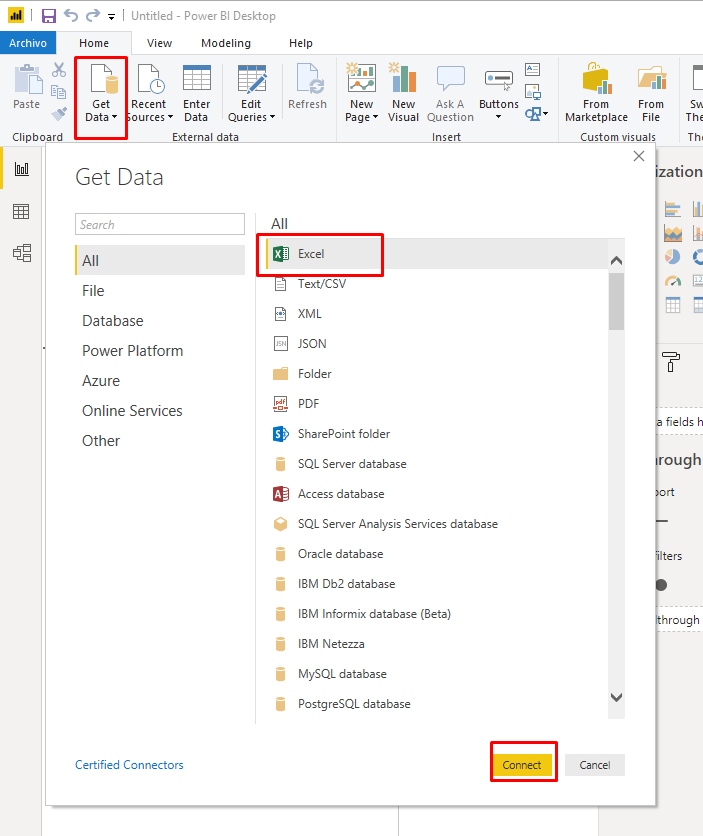
\includegraphics[scale=0.5]{./Imagenes/image001}
\item 4. En el cuadro de dialogo Abrir (Open), buscar el archivo Adventure Works Sales Data.xlsx, y luego hacer click en Abrir (Open).
\item 5. En el cuadro de dialogo Explorador (Navigator), seleccionar las hojas DimCurrency, DimCustomer,DimDate, DimProduct, DimPromotion, DimSalesTerritory, y FactInternetSales.
\item 6. Hacer click en Cargar (Load). \\
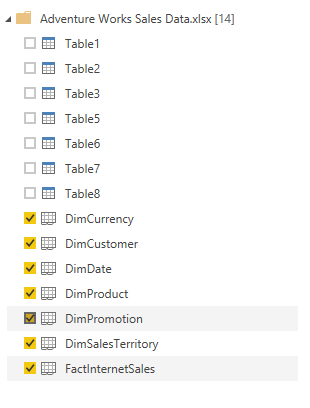
\includegraphics[scale=0.5]{./Imagenes/image002}
\item 7.En el panel de vistas a mano derecho, hacer click en Relaciones (Relationships).
\item 8.En el menú principal, hacer click en Administrar relaciones (Manage Relationships).
\item 9. En el cuadro de Administrar relaciones (Manage Relationships), hacer click en Nueva (New). \\
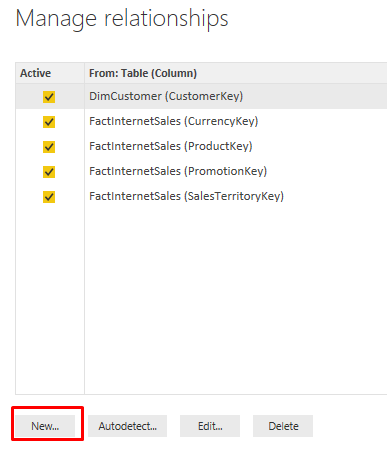
\includegraphics[scale=0.5]{./Imagenes/image003}
\item 10.En el cuadro de Administrar relaciones (Manage Relationships), en la lista de tablas superior, hacer click en FactInternetSales. Cuando la vista previa de la table aparezca hacer click en la columna OrderDateKey.
\item 11. En la lista de table inferior, hacer click en DimDate. Cuando la vista previa de la table aparezca hacer click en la columna DateKey.
\item 12. Revisar que la cardinalidad (Cardinality) esta seleccionada para Muchos a Uno (Many to One (*:1)), que la Dirección del filtro cruzado (Cross filter direction) es Sencilla (Single), y que la opción Hacer esta relaciónactiva (Make this relationship active) se encuentra seleccionada, luego hacer click en Aceptar (OK).
\item 13. En el cuadro de Administrar relaciones (Manage Relationships), hacer click en Cerrar (Close). \\
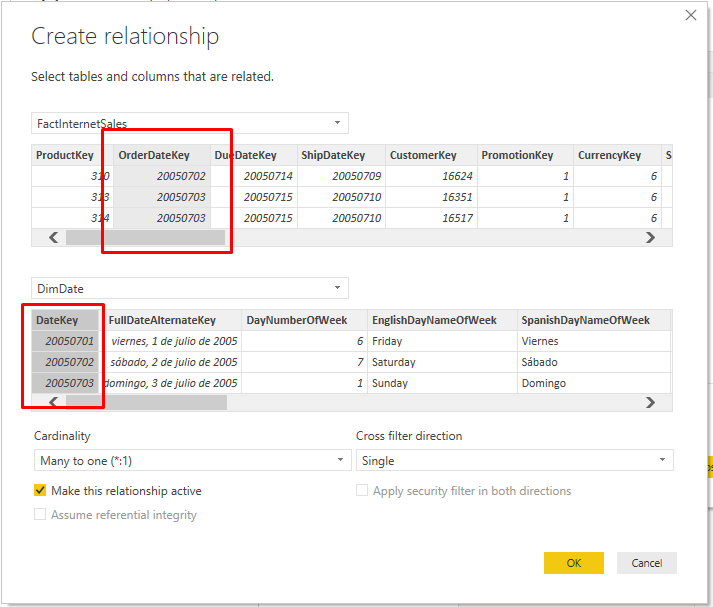
\includegraphics[scale=0.5]{./Imagenes/image004}
\item 14.En el diagrama, en la tabla FactInternetSales, hacer click en la columna DueDateKey. Arrastrar la columna DueDateKey a la columna DateKey de la tabla DimDate.
\item 15. En el diagrama, en la tabla FactInternetSales, hacer click en la columna ShipDateKey. Arrastrar la columna ShipDateKey a la columna DateKey de la tabla DimDate. \\
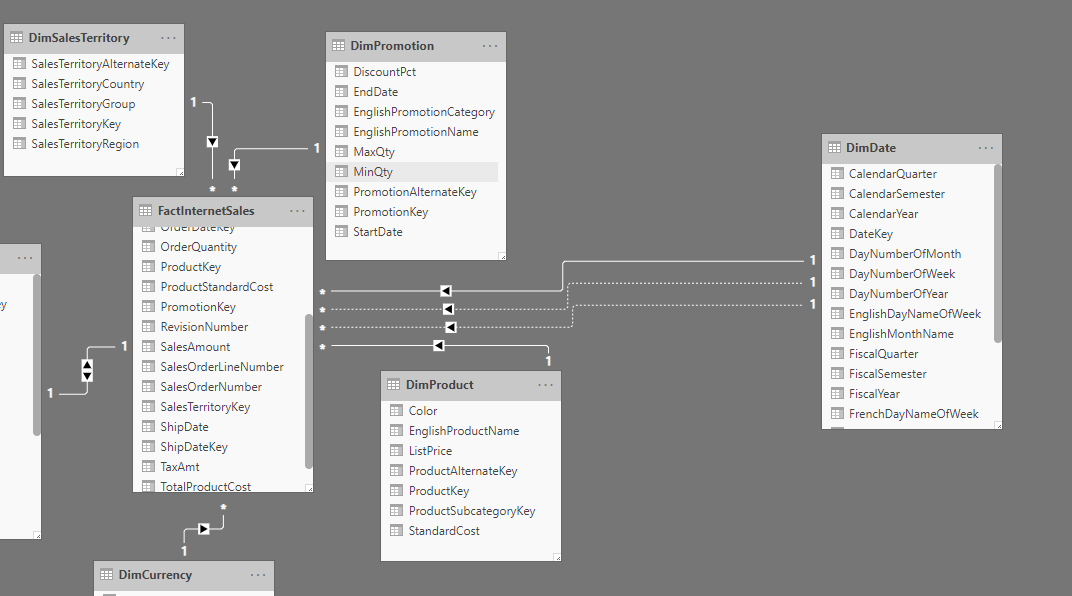
\includegraphics[scale=0.5]{./Imagenes/image005}
\item 16. En el menú principal, hacer click en Administrar relaciones (Manage Relationships).
\item 17. En el cuadro de Administrar relaciones (Manage Relationships), hacer doble click en la relación FactInternetSales (CurrencyKey). \\
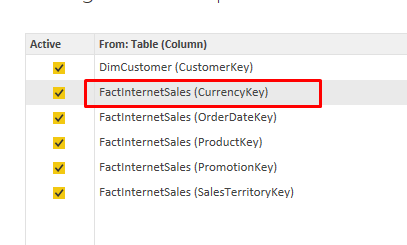
\includegraphics[scale=0.5]{./Imagenes/image006}
\item 18. En la lista de Dirección de Filtro Cruzado (Cross filter direction), hacer click en Sencilla (Single), luego hacer click en Aceptar (OK).
\item 19. En el cuadro de Administrar relaciones (Manage Relationships), hacer doble click en la relación FactInternetSales (ProductKey).
\item 20. En la lista de Dirección de Filtro Cruzado (Cross filter direction), hacer click en Sencilla (Single), luego hacer click en Aceptar (OK).
\item 21. En el cuadro de Administrar relaciones (Manage Relationships), hacer doble click en la relación FactInternetSales (PromotionKey).
\item 22. En la lista de Dirección de Filtro Cruzado (Cross filter direction), hacer click en Sencilla (Single), luego hacer click en Aceptar (OK).\\
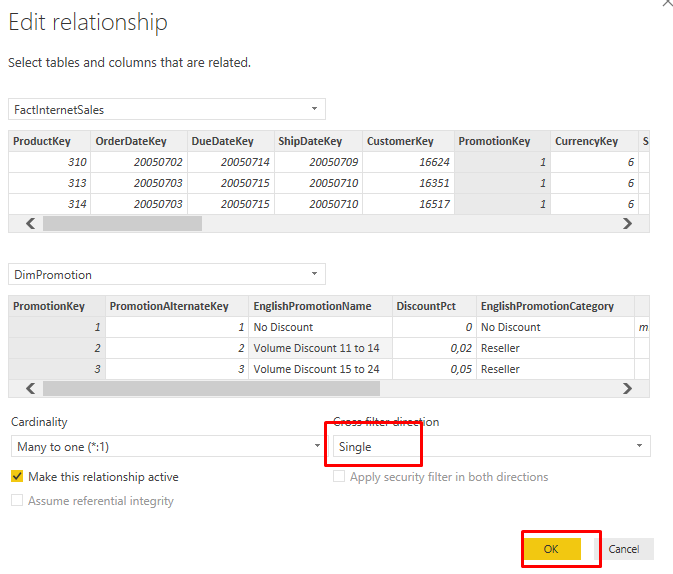
\includegraphics[scale=0.5]{./Imagenes/image007}
\item 23. En el cuadro de Administrar relaciones (Manage Relationships), hacer doble click en la relación FactInternetSales (SalesTerritoryKey).
\item 24. En la lista de Dirección de Filtro Cruzado (Cross filter direction), hacer click en Sencilla (Single), luego hacer click en Aceptar (OK). \\
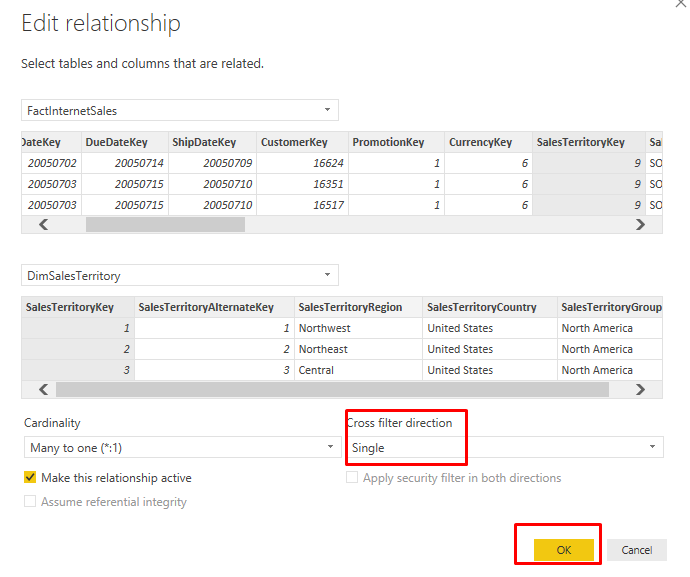
\includegraphics[scale=0.5]{./Imagenes/image008}
\item 25. En el cuadro de Administrar relaciones (Manage Relationships), hacer click en Cerrar (Close)..
\item 26. Hacer click en la línea de relación entre FactInternetSales and DimCustomer y presionar Borrar (Delete).
\item 27. En el cuadro de dialogo Eliminar relación (Delete Relationship), hacer click en Borrar (Delete).\\
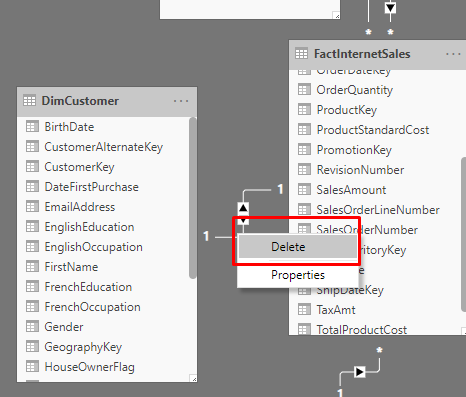
\includegraphics[scale=0.5]{./Imagenes/image009}
\item 28. En el menú principal, hacer click en Administrar relaciones (Manage Relationships).
\item 29. En el cuadro de Administrar relaciones (Manage Relationships), hacer click en Nueva (New).
\item 30. En la lista de tablas superior, hacer click en FactInternetSales. Luego hacer click en la columna CustomerKey en la vista de datos previa.
\item 31. En la lista de tablas superior, hacer click en DimCustomer, y hacer click CustomerKey en la vista de datos previa.
\item 32. En la lista de Cardinalidad (Cardinality), hacer click en Muchos a Uno (Many to One (*:1)), y luego hacer click en Aceptar (OK). \\
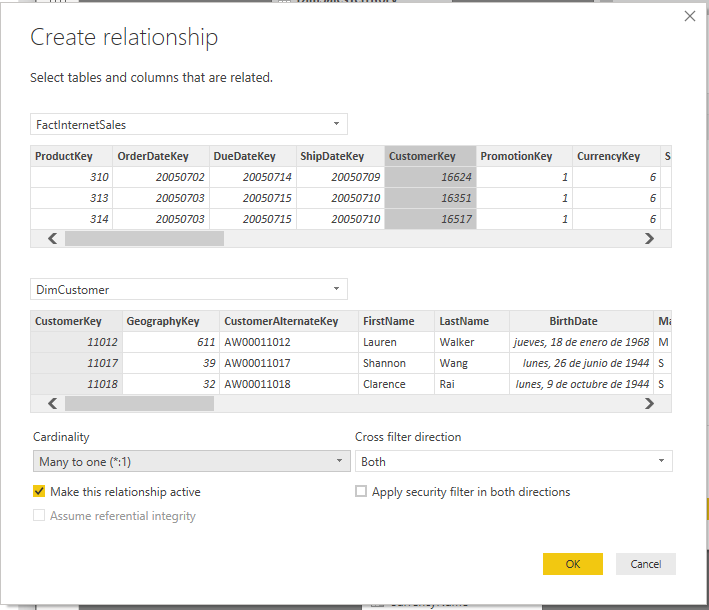
\includegraphics[scale=0.5]{./Imagenes/image010}
\item 33. En el cuadro de Administrar relaciones (Manage Relationships), hacer click en Cerrar (Close).
\item 34. Hacer click en Guardar (Save), y cuargar el archive como Ventas Adventure Works.pbix.\\
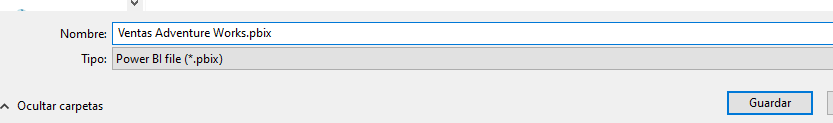
\includegraphics[scale=0.5]{./Imagenes/image011}

\subsection {TAREA 2:  RELACIONES MANUALES}
\item 1. En la Ventana de Power BI Desktop, click en Obtener Datos (Get Data) y luego en Excel
\item 2. Abrir el archivo Adventure Works Product Categories.xlsx.
\item 3. En el cuadro de dialogo Explorador (Navigator), seleccionar las hojas DimProductCategory, andDimProductSubcategory, y luego hacer click en Cargar (Load).\\
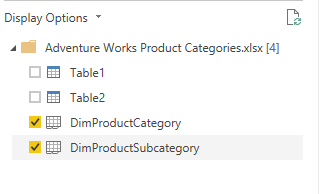
\includegraphics[scale=0.5]{./Imagenes/image012}
\item 4. En el panel de Relaciones, revisar la relación que Power BI ha creado entre las dos tablas.
\item 5. Hacer click en la línea de la relación entre DimProductCategory, y DimProductSubcategory, y seleccionar Eliminar (Delete). \\
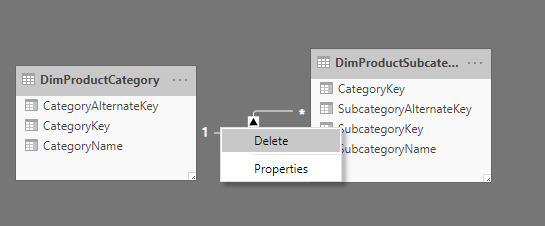
\includegraphics[scale=0.5]{./Imagenes/image013}
\item 6. En el cuadro de dialogo Eliminar relación (Delete Relationship), hacer click en Borrar (Delete).
\item7. Arrastrar la columna CategoryKey en la tabla DimProductSubcategory a la columna Category en la tabla DimProductCategory, para crear una relación Muchos a uno (Many to One (*:1)), y una dirección de filtro cruzado (Cross filter direction) en ambos.
\item 8. En la tabla DimProduct, arrastrar la columna ProductSubcategoryKey a la columna SubcategoryKey en la tabla DimProductSubcategory, para crear una relación de Muchos a Uno (Many to One (*:1)), y una dirección de filtro cruzado (Cross filter direction) en ambos.
\item9. Hacer click en Guardar \\
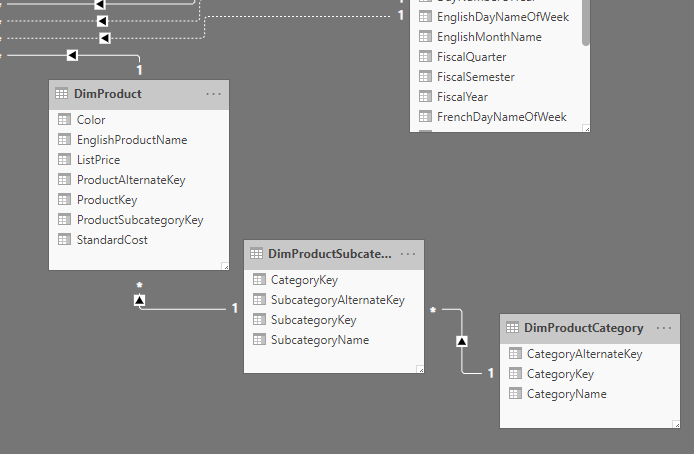
\includegraphics[scale=0.5]{./Imagenes/image014}


\end{itemize}
\section{CALCULOS} 
\subsection{AGREGAR UNA COLUMNA CALCULADA}

\begin{itemize}

\item 1. En Power BI Desktop, haga clic en Datos en el panel de vistas en el lado izquierdo.
añadir el control al reporte.
\item 2. En el panel Campos, haga clic en DimCustomer.
\item 3. En la cinta de Modelado, en el grupo Cálculos, haga clic en Nueva columna.\\
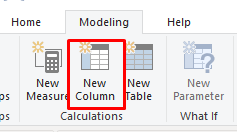
\includegraphics[scale=0.5]{./Imagenes/image015}
\item 4. En la barra de fórmulas, resalte Columna = y escriba: \\
IncomeStatus = IF (DimCustomer[YearlyIncome] < 25000, "Lower Income",\\
IF (AND(DimCustomer[YearlyIncome] >= 25000, DimCustomer[YearlyIncome] < 60000),\\
"Middle Income",\\
IF (AND(DimCustomer[YearlyIncome] >= 60000, DimCustomer[YearlyIncome] < 100000),\\
"Higher Income",\\
IF (DimCustomer[YearlyIncome] >= 100000, "Very High Income", "Other")))) \\

\item 5. Presione Enter. \\
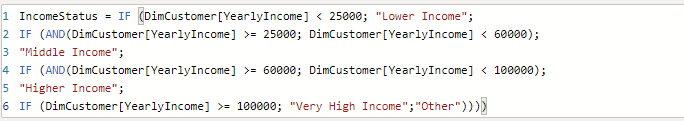
\includegraphics[scale=0.5]{./Imagenes/image016}
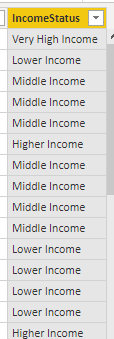
\includegraphics[scale=0.5]{./Imagenes/image017}

\item 6. En la cinta de Modelado, en el grupo Cálculos, haga clic en Nueva columna.
\item 7. En la barra de fórmulas, resalte Columna = y escriba: \\
DaysSinceFirstPurchase = DATEDIFF(DimCustomer[DateFirstPurchase], TODAY(), DAY) \\
\item 8. Presione Enter. \\

\includegraphics[scale=0.5]{./Imagenes/image018}
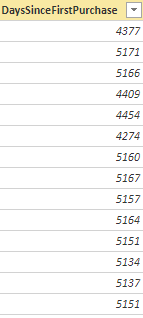
\includegraphics[scale=0.5]{./Imagenes/image019}
\item 9. En la cinta de Modelado, en el grupo Cálculos, haga clic en Nueva columna.

\item 10. En la barra de fórmulas, resalte Columna = y escriba: \\
FullName = [FirstName] [LastName] \\

\item 11. Presione Entrar. \\


\includegraphics[scale=0.5]{./Imagenes/image020}
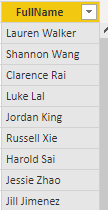
\includegraphics[scale=0.5]{./Imagenes/image021}

\item 12. En la cinta de Modelado, en el grupo Cálculos, haga clic en Nueva columna.
\item 13. En la barra de fórmulas, resalte Columna = y escriba:\\
MaleFemale = IF ([Gender] = "M", "Male", "Female")

\item14. Presione Entrar.\\
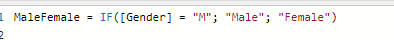
\includegraphics[scale=0.5]{./Imagenes/image022}
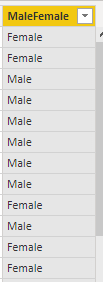
\includegraphics[scale=0.5]{./Imagenes/image023}

\item 15. En la cinta de Modelado, en el grupo Cálculos, haga clic en Nueva columna.

\item 16. En la barra de fórmulas, resalte Columna = y escriba:\\
Relationship = IF([MaritalStatus] = "M", "Married", "Single")\\
\item 17. Presione Entrar. \\
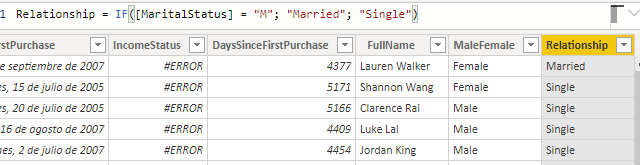
\includegraphics[scale=0.5]{./Imagenes/image024}
\item 18. En el panel Campos, haga clic en DimProductSubcategory.

\item 19. En la cinta de Modelado, en el grupo Cálculos, haga clic en Nueva columna.

\item 20. En la barra de fórmulas, resalte Columna = y escriba:\\
MainCategory = RELATED (DimProductCategory [CategoryName])
\\
\item 21. Presione Entrar.\\
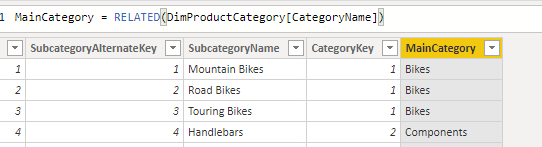
\includegraphics[scale=0.5]{./Imagenes/image025}
\item 23. En la cinta de Modelado, en el grupo Cálculos, haga clic en Nueva columna.
\item 24. En la barra de fórmulas, resalte Columna = y escriba:\\
PromotionLengthDays = DATEDIFF (DimPromotion [StartDate], DimPromotion [EndDate], DAY)\\

\item 25. Presione Entrar.\\
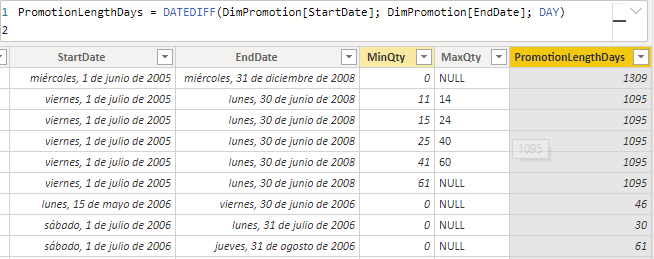
\includegraphics[scale=0.5]{./Imagenes/image026}
\item 26. En el panel Campos, haga clic en FactInternetSales.
\item 27. En la cinta de Modelado, en el grupo Cálculos, haga clic en Nueva columna.
\item 28. En la barra de fórmulas, resalte Columna = y escriba:\\
Profit = CURRENCY(FactInternetSales[UnitPrice] - \\
FactInternetSales[ProductStandardCost])\\
\item 29. Pressionar Enter.\\
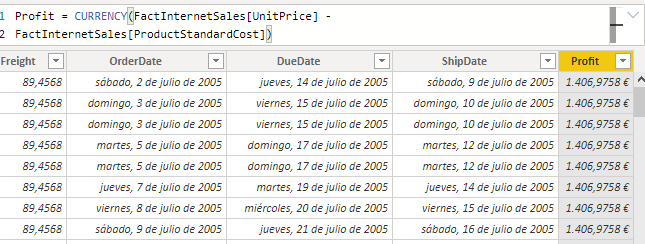
\includegraphics[scale=0.5]{./Imagenes/image027}
\item 30. Cerrar Power BI Desktop, salvando cualquier cambio. \\
LINK: https://app.powerbi.com/groups/me/reports/9800665a-badd-4100-a74f-4fea5114c745/ReportSection

\end{itemize}


\end{document}
